For et henfald, hvor moderkernen deles i to, et såkaldt to-partikelhenfald {$M \rightarrow a + b$},
er der otte frihedsgrader - to impulsvektorer, hver med tre komponenter, samt to energier. Disse
størrelser er underlagt bevarelseslovene for energi og impuls, hvilket reducerer antallet af
frihedsgrader til nul. I et energispektrum vil et sådant henfald give anledning til to
toppe. Energierne af disse i massemidtpunktssystemet for moderkernen er givet ved
\begin{equation}
  \label{eq:toE}
  T_{a} = \frac{m_{b}}{m_{a} + m_{b}}Q, \qquad T_{b} = \frac{m_{a}}{m_{a} + m_{b}}Q.
\end{equation}

Tre-partikelhenfaldet, {$M \rightarrow a + b + c$}, har derimod 12 frihedsgrader - ni fra impuls og
tre fra energi. Dette kan reduceres ved at overveje følgende; henfaldet foregår i ét plan, så
$p_{i,z}$ kan sættes lig nul. Dette fjerner tre frihedsgrader. Energi- og impulsbevarelse eliminerer
tilsammen tre frihedsgrader. Energi-impuls relationen, $E^{2} = p^{2} + m^{2}$, anvendt for hver
enkelt datterkerne begrænser også tre frihedsgrader. En rotation i xy-planet ændrer ikke systemet,
hvilket fjerner én enkelt frihedsgrad. Antallet af frihedsgrader kan dermed reduceres til to,
hvilket betyder, at systemets tilstand afgøres af dynamikken, dvs. vekselvirkninger i systemet.

Henfalder \Carb-kernen direkte til tre ikke-vekselvirkende $\alpha$-partikler, vil energispektret
pga. de to frihedsgrader udgøre et kontinuum af energier. Denne proces kaldes direkte henfald og
er skitseret på \cref{fig:becker}a.

\begin{figure}
  \centering
  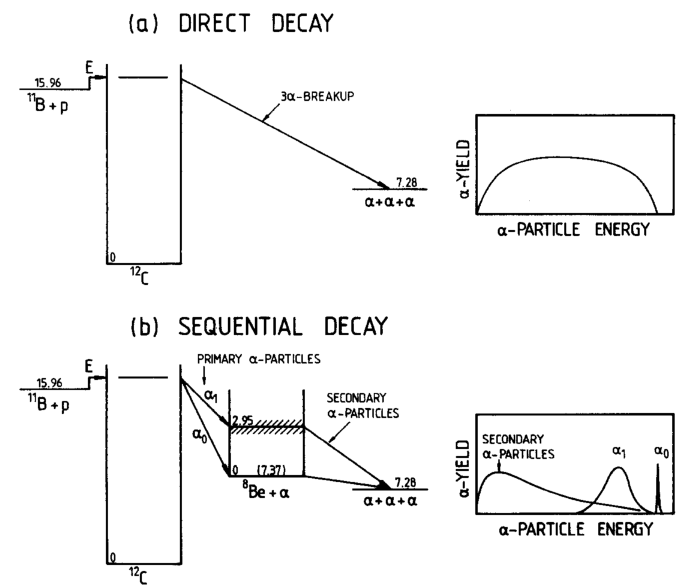
\includegraphics{Becker}
  \caption{Energidiagram for henfaldsprocessen af \Carb skitseret for hhv. (a) direkte henfald  og
    (b) sekventielt henfald. Figuren er lånt fra \cite{becker}.}
  \label{fig:becker}
  \vspace{-5mm}
\end{figure}
